

\documentclass[8pt]{beamer}
\mode<presentation>
\linespread{1.5}

\usetheme{Madrid}
%\usetheme {CambridgeUS}%{Goettingen}%{Berkeley}%{Montpellier}%{Antibes}%{Dresden}%{Madrid}%{Dresden}%{Darmstadt}%{Warsaw}%{Pittsburgh}
\usefonttheme{{structuresmallcapsserif}}%{structureitalicserif}%{structurebold}%{structuresmallcapsserif}%{professionalfonts}
%\useoutertheme[subsection=false]{smoothbars}
\usepackage[english]{babel}
%\usepackage[latin1]{inputenc}
\usepackage{hyperref}
%\usecolortheme{beaver}
%\usecolortheme{crane}

%\setbeamercovered{transparent}
%\newcommand{\semitransp}[2][35]{\color{fg!#1}#2}

\usepackage{latexsym}
\usepackage{amsmath}
\usepackage{times}
%\usepackage{MinionPro}
\usepackage{hyperref}
\usepackage{tikz}
\usepackage{verbatim}
\usepackage{natbib}
\usepackage{color, colortbl}
\usepackage{appendix}
\usepackage{ulem}
\usepackage{amsmath,amsthm}
\usepackage{bbm}
\usetikzlibrary{arrows,shapes}


\newtheorem{proposition}{Proposition}[section]
%\newtheorem{definition}{Definition}[section]
\newtheorem{assumption}{Assumption}[section]
\newtheorem{conjecture}{Conjecture}[section]
\newtheorem*{observation}{Observation}


\definecolor{Gray}{gray}{0.9}


\pgfdeclarelayer{background}
\pgfsetlayers{background,main}

\tikzstyle{vertex}=[circle,fill=black!25,minimum size=12pt,inner sep=0pt]
\tikzstyle{selected vertex} = [vertex, fill=red!24]
\tikzstyle{unknown vertex} = [vertex, fill=black]
\tikzstyle{edge} = [draw,thick,-]
\tikzstyle{weight} = [font=\small]
\tikzstyle{selected edge} = [draw,line width=5pt,-,red!50]
\tikzstyle{ignored edge} = [draw,line width=5pt,-,black!20]







\title{Coordination in Social Networks}
\author{Chun-Ting Chen}


\begin{document}

\maketitle


\section{Introduction}
\subsection{Motivation}


\frame{
  \frametitle{Motivation}

\begin{itemize}
\item The relevant information in making joint decision is dispersed in the society. (Hayek 1945)
\item If so, how people act collectively?
\begin{itemize}
\item Ex.: protest, currency attack, joint investment, etc.
\end{itemize}
\end{itemize}



%\begin{quote}
%never exists in concentrated or integrated form, but solely as the dispersed bits of incomplete and frequently contradictory knowledge which all the separate individuals possess.
%\end{quote}

}


\frame{
  \frametitle{This paper shows}

\begin{itemize}
\item In a long-term relationship, people can aggregate such information and coordinate their actions.
\end{itemize}



%\begin{quote}
%never exists in concentrated or integrated form, but solely as the dispersed bits of incomplete and frequently contradictory knowledge which all the separate individuals possess.
%\end{quote}

}


\frame{
  \frametitle{What this paper does?}

\begin{itemize}
\item I model a repeated game with \underline{incomplete information and network-monitoring}.
\begin{itemize} 
\item Players can only observe own/neighbors' \textcolor{blue}{types} and own/neighbors' \textcolor{blue}{actions}. 
\end{itemize} 
\item Look for an equilibrium in which the pay-off relevant information become \underline{commonly known in finite time}.
\begin{itemize}
\item A strong requirement.
\end{itemize}
\item Such equilibrium can be constructed under some assumptions.
\end{itemize}

}


\frame{
  \frametitle{Related literature}

\begin{itemize}
\item Strategic learning in repeated game with incomplete information
\begin{table}[h]
\begin{tabular}{lll}
& without discount factor & with discount factor \\
\hline
\textcolor{blue}{perfect monitoring}  &  [Forges 1992]$^{*}$, etc &  [Jordan 1995],[Peski 2014]$^{*}$, etc \\
\\
\textcolor{blue}{imperfect monitoring} & [Aumann and Maschiler 1990], etc & \\
network-monitoring & [Renault and Tomala 1998], etc & \alert{This paper}
\end{tabular}
\end{table}
\item Collective action: [Chwe 2000]$^{*}$, [Morris and Shin 1998], etc. 
\end{itemize}

}


\section{Model}
\subsection{Model}

\frame{
  \frametitle{Model}
Time line

\begin{enumerate}


\item There is a \alert{fixed}, \alert{finite}, \alert{connected}, \alert{undirected}, and \alert{commonly known} network.
\item Players of two types--- \textit{S} or \textit{B} ---chosen by nature according to a probability distribution.
\item Types are then fixed over time.
\item Players play a stage game--- a collective action ---infinitely repeatedly with common discount factor.
\end{enumerate}



}


\begin{frame}
  \frametitle{Model}

What player can/cannot observe

\begin{itemize}
\item Players can observe own/neighbors' \textcolor{blue}{types} and \textcolor{blue}{actions}, but not others'.
\item Pay-off is hidden.
\begin{itemize}
\item Viewing the pay-off as the expected pay-off:  [Aumann and Maschiler 1990], [Miyahara and Sekiguchi 2013], [Wolitzky 2013], etc.
\end{itemize}
\end{itemize}




\end{frame}


\begin{frame}
  \frametitle{Model}

  \begin{itemize}

  \item Stage game---\alert{$k$}-threshold game: a \textcolor{blue}{protest} (~[Chwe 2000])




\begin{itemize}
\item S-type's action set$=\{\textbf{p},\textbf{n}\}$
\item B-type's action set$=\{\textbf{n}\}$
\item (Expected) pay-offs for S-type:
\begin{table}[h]
\begin{tabular}{llll}
$u_{S_i}(a_{S_i},a_{-\theta_i})$ & $=$ & 1 & if $a_{S_i}=\textbf{p}$ and $\#\{j:a_{\theta_j}=\textbf{p}\}\geq {k}$ \\
$u_{S_i}(a_{S_i},a_{-\theta_i})$ & $=$ & -1 & if $a_{S_i}=\textbf{p}$ and $\#\{j:a_{\theta_j}=\textbf{p}\}< {k}$ \\
\\
$u_{S_i}(a_{S_i},a_{-\theta_i})$ & $=$ & 0 & if $a_{S_i}=\textbf{n}$ 
\end{tabular}

\end{table}
\end{itemize}
  

 \end{itemize}

\end{frame}



\begin{frame}
  \frametitle{Static ex-post Pareto efficient outcome}



\begin{table}[h]
\begin{tabular}{ll}
Type profile & Static ex-post efficient outcome \\
\hline
At least $k$ S-types exist & All S-types play \textbf{p}  \\
Otherwise &  All S-types play \textbf{n} 
\end{tabular}
\end{table}
\end{frame}




\begin{frame}
  \frametitle{Equilibrium concept}

\begin{itemize}
\item WPBE (weak perfect Bayesian equilibrium)
\item Sequential equilibrium
\end{itemize}
\end{frame}


\begin{frame}
  \frametitle{APEX equilibrium}

\textcolor{blue}{APEX} (\textit{approaching ex-post efficient}) equilibrium

\begin{definition}[APEX strategy]
An equilibrium is APEX $\Leftrightarrow$ 
\[\text{$\forall\theta$,  there is a finite time $T^{\theta}$}\] 
such that the actions in the equilibrium path repeats the static ex-post efficient outcome after $T^{\theta}$. 
\end{definition}

\end{frame}










%\begin{frame}
%  \frametitle{Notations}
%
%Notations:
%\begin{itemize}
%
%\item $\alert{\theta_{G_i}}\in \Theta_{G_i}$: $i$'s private information about the state. 
%\item $\alert{h^{m}_{G_i}}\in H^m_{G_i}$: the history of actions observed by $i$ up to period $m$.
%\item \alert{$\Theta_{G_i}\times H^m_{G_i}$}: $i$'s observation up to time $m$.
%\pause
%\item $h^m$: a sequence of players' actions up to period $m$.
%\item $h$: an infinite sequence of players' actions. 
%
%
%
%
% 
%\end{itemize}
%
%\end{frame}
%
%
%
%
%\begin{frame}
%  \frametitle{APEX strategy path}
%Notations:
%\begin{itemize}
%\item $\tau_i:\Theta_{G_i}\times \bigcup^{\infty}_{m=0} H^{m}_{G_i} \rightarrow A_{\theta_i}$, $i$'s strategy.
%\item $\tau=(\tau_1,...,\tau_i,...,\tau_n)$: a strategy profile. 
%\item $h^{\tau}_{\theta}$ : a history generated by $\tau$ given $\theta$.
%\item $\tau$-path: $\{h^{\tau}_{\theta}\}_{\theta\in \Theta}$
%\end{itemize}
%
%\begin{definition}
%The $\tau$-path is \textbf{approaching ex-post efficient} (\textcolor{blue}{\textit{APEX}}) $\Leftrightarrow$ 
%\[\text{$\forall\theta$,  there is a finite time $T^{\theta}$}\] 
%such that the actions after $T^{\theta}$ in $h^{\tau}_{\theta}$ repeats the static ex-post efficient outcome.
%\end{definition}
%
%
%\end{frame}
%
%
%
%
%\begin{frame}
%  \frametitle{Equilibrium Concept}
%
%Notations:
%\begin{itemize}
%
%\item $\beta^{\pi,\tau}_i(\theta|h^{m}_{G_i})$: $i$'s belief for a $\theta$ at period $m$ given $\pi,\tau$.
%\item $\phi_{G_i}: H^m\rightarrow H^m_{G_i}$: the projection mapping a $h^m$ to $h^m_{G_i}$.
%\end{itemize}
%
%\begin{definition}
%$h^m_{G_i}$ is \textbf{reached} by $\tau$ iff there is a pair $(\theta,h^m)$ such that $h^m$ is on the $\tau$-path, and $h^m_{G_i}=\phi_{G_i}(h^m)$. 
%\end{definition}
%
%
%\end{frame}
%
%
%\begin{frame}
%  \frametitle{Equilibrium Concept}
%
%
%\begin{definition}[weak sequential equilibrium]
%The pair $(\tau^{*},\beta^{*})$, 
%\begin{itemize}
%\item $\tau^{*}$: a strategy
%\item $\beta^{*}=\{\beta^{*,m}\}_m$: the belief system 
%\begin{itemize}
%\item $\beta^{*,m}_i$: $\Theta_{G_i}\times H^{m}_{G_i} \rightarrow \Delta (\Theta\times H^m)$
%\end{itemize}
%\end{itemize}
%
%, is a weak sequential equilibrium iff
%\begin{itemize}
%\item $\beta^{*,m}_i(\theta|h^{m}_{G_i})=\beta^{\pi,\tau^{*}}_i(\theta|h^{m}_{G_i})$ whenever $h^{m}_{G_i}$ is reached by $\tau^{*}$ for all $i$.
%\item $\tau^{*}$ is sequential rational given $\beta^{*}$.
%\end{itemize}
%
%
%
%
%
%\end{definition}
%
%
%
%
%\end{frame}
%
%
%\begin{frame}
%  \frametitle{Equilibrium Concept}
%
%
%\begin{definition}[Sequential equilibrium]
%A sequential equilibrium $(\tau^{*},\beta^{*})$  is a weak  sequential equilibrium and $\beta^{*}$ is fully consistent with $\tau^{*}$[Krep and Wilson].
%\end{definition}
%\begin{itemize}
%\item Fully consistent: 
%the $\beta^{*}$ is \textbf{``very very similar with''} that belief system induced by a \textbf{``very very little perturbed''} strategies around $\tau^{*}$.
%\end{itemize}
%\end{frame}
%
%\begin{frame}
%  \frametitle{APEX Equilibrium}
%
%\begin{itemize}
%\item Finally, let the ``(weak) APEX equilibrium'' be \textcolor{blue}{the (weak) sequential equilibrium in which the equilibrium path is APEX}.
%\item Does an APEX equilibrium exist?
%\end{itemize}
%
%\end{frame}
%


\frame{
  \frametitle{Result 1: APEX for $k=n$}

\begin{theorem}[\alert{$k=n$}]

If $k=n$, then an APEX sequential equilibrium exists whenever discount factor is sufficiently high.
\end{theorem}


}


\begin{frame}
  \frametitle{Definition for APEX for $k<n$}


\begin{definition}
$\theta$ has \textbf{strong connectedness}$\Leftrightarrow$ for every pair of S-types, there is a path consisting of S-types to connect them.
\end{definition}  

\begin{definition}
$\pi$ has \textbf{full support on strong connectedness}$\Leftrightarrow$ 
\[\text{$\pi(\theta)>0$ \textbf{if and only if} $\theta$ has strong connectedness.}\]
\end{definition}  


\end{frame}


\begin{frame}
  \frametitle{Without strong connectedness}
Let k=\alert{2} and n=\alert{3}
\begin{center}
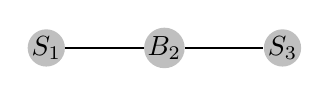
\begin{tikzpicture}[scale=1.5]
    % Draw a 7,11 network
    % First we draw the vertices
    \foreach \pos/\name in {{(1,0)/S_1}, {(2,0)/B_2}, {(3,0)/S_3}}
        \node[vertex] (\name) at \pos {$\name$};
    % Connect vertices with edges 
    \foreach \source/ \dest in {S_1/B_2, B_2/S_3}
        \path[edge] (\source) -- (\dest) ;
        
\end{tikzpicture}
\end{center}

\begin{itemize}


\item A B-type will not reveal information.
\item \textbf{Without} {full support on strong connectedness}, in general, an Apex equilibrium does not exist when pay-off is hidden.

\end{itemize}
\end{frame}


\frame{
  \frametitle{Result 2: APEX for $k<n$}

\begin{theorem}[\alert{$k< n$}]
If $k<n$, then if network is a \alert{tree}, if prior $\pi$ has \alert{full support on strong connectedness}, then an APEX WPBE {exists} whenever discount factor is sufficiently high.
\end{theorem}

}

\begin{frame}


  \frametitle{Outline for Equilibrium Construction}

\begin{enumerate}

\item APEX sequential equilibrium for $k=n$.
\begin{itemize}
\item An example.
\item Sketch of proof.
\end{itemize}
\item APEX WPBE for $k<n$.
\begin{enumerate}
\item Consider cheap talk.
\item Consider ``costly'' talk.
\item Sketch of proof.
\end{enumerate}
\end{enumerate}


\end{frame}



\begin{frame}
  \frametitle{An example for $k=n$}
\begin{center}
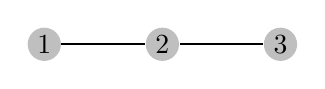
\begin{tikzpicture}[scale=1.5]
    % Draw a 7,11 network
    % First we draw the vertices
    \foreach \pos/\name in {{(1,0)/1}, {(2,0)/2}, {(3,0)/3}}
        \node[vertex] (\name) at \pos {$\name$};
    % Connect vertices with edges 
    \foreach \source/ \dest in {1/2, 2/3}
        \path[edge] (\source) -- (\dest) ;
        
\end{tikzpicture}
\end{center}

  
Let \alert{$k=n=3$}, when discount factor is high enough, an APEX sequential equilibrium can be constructed by
\begin{itemize}

\item \textcolor{blue}{Period 1}
\begin{itemize}
\item S-type 2: choose $\textbf{p}$ if $\theta=(S,S,S)$;
\item S-type 2: choose $\textbf{n}$ if $\theta\neq (S,S,S)$, and then choose \alert{\textbf{n} forever}.
\item S-type 1 (or S-type 3): \textbf{p}.
\end{itemize}

\item \textcolor{blue}{Period 2}
\begin{itemize}
\item If S-type 2 chooses \textbf{p} in the last period $\Rightarrow$ S-type 1 (or S-type 3) chooses \textbf{p} forever; 
\item If S-type 2 chooses \textbf{n} in the last period $\Rightarrow$ S-type 1 (or S-type 3) chooses \alert{\textbf{n} forever}.
\end{itemize}
 
 \item Any deviation $\Rightarrow$ Choosing \alert<1->{\textbf{n} forever}.
\end{itemize}

\end{frame}


\begin{frame}
  \frametitle{An example for $k=n$}
Main features in equilibrium construction in this example
\begin{itemize}
\item The \alert{1st-period} actions serve as ``\textcolor{blue}{messages}'' to reveal the relevant information.
\item The \alert{2nd-period} is a commonly known ``\textcolor{blue}{timing}'' to coordinate (part of equilibrium strategy).
\item \alert{Playing \textbf{n} forever} serves as a ``\textcolor{blue}{grim trigger}''.
\end{itemize}  
\end{frame}



\section{Equilibrium construction}
\subsection{Equilibrium construction}

\frame{
  \frametitle{Equilibrium construction for \alert{$k=n$}}


Sketch of proof:
  \begin{enumerate}
  
\item ``messages'' to reveal the relevant information.
\begin{itemize}
  \item Some B-types neighbors $\Rightarrow$ play \textbf{n} forever.
  \item No B-type neighbor $\Rightarrow$ play \textbf{p} unless \textbf{n} is observed, and then play \textbf{n} forever.
\end{itemize}
\pause
\item ``Timing'' to coordinate.
\begin{itemize}
 \item Finite network $\Rightarrow$ there is a finite time $T$ such that players coordinate to the static ex-post efficient outcome.
\end{itemize}
 \pause
  \item Any deviation $\Rightarrow$ play ``\textbf{n} forever''.
  \pause
  \item A belief system for sequential equilibrium can be chosen.
   \end{enumerate}

}















\frame{
  \frametitle{Equilibrium construction for \alert{$k<n$}}

\begin{center}
\begin{tikzpicture}%[
%    thick,
%    >=stealth',
%    dot/.style = {
%      draw,
%      fill = white,
%      circle,
%      inner sep = 0pt,
%      minimum size = 4pt
%    }
%  ]

  \draw[->] (0,0) -- (8,0); %coordinate[label = {below:$x$}] (xmax);
  \draw[-] (4,-0.1) -- (4, 0.1) node [above]{$T$(?)};
 

\end{tikzpicture}
\end{center}


\begin{itemize}
\item Challenges:
\begin{itemize}
\item How to find that finite time ``$T$'' for every state?
\item Only two actions used for transmit relevant information.
\item Group punishment is hard to be made. (Network-monitoring)
\end{itemize}

\end{itemize}

}


\frame{
  \frametitle{Equilibrium construction for \alert{$k<n$}}
\begin{center}
\begin{tikzpicture}%[
%    thick,
%    >=stealth',
%    dot/.style = {
%      draw,
%      fill = white,
%      circle,
%      inner sep = 0pt,
%      minimum size = 4pt
%    }
%  ]

  \draw[->] (0,0) -- (8,0); %coordinate[label = {below:$x$}] (xmax);
  \draw[-] (4,-0.1) -- (4, 0.1) node [above]{$T$(?)};
 

\end{tikzpicture}
\end{center}
\[\downarrow\]
\begin{center}
\begin{tikzpicture}%[
%    thick,
%    >=stealth',
%    dot/.style = {
%      draw,
%      fill = white,
%      circle,
%      inner sep = 0pt,
%      minimum size = 4pt
%    }
%  ]

  \draw[->] (0,0) -- (4,0); %coordinate[label = {below:$x$}] (xmax);
  \draw[-] (4,-0.1) -- (4, 0.1) node [above]{$T$};
 

\end{tikzpicture}
\end{center}

\begin{itemize}
\item By definition of APEX,
\begin{itemize}
\item After $T$, actions are infinitely repeated and thus information can not be updated. 
\end{itemize}

\item Idea:
\begin{enumerate}
\item Assume $T$ is fixed, commonly known, and independent from states. 
\item Players can transmit information by ``talking'' only within $T$ rounds.
\begin{itemize}
\item Consider an augmented $T$-round ``cheap talk'' phase.
\item Consider an augmented $T$-round ``costly talk'' phase.
\end{itemize}
\end{enumerate}
\end{itemize}

}

\begin{frame}
  \frametitle{$k$-Threshold game augmented by $T$-round cheap talk}

Time line
\begin{itemize}

\item Nature choose $\theta$ according to $\pi$.
\item Types are then fixed over time.
\item At the first $T$ rounds, players play $T$-round cheap talk.
\item At $T+1$ round, players play a one-shot $k$-Threshold game.
\item Game ends.
\end{itemize}

\end{frame}






\begin{frame}
  \frametitle{$k$-Threshold game augmented by $T$-round cheap talk}

\begin{itemize}
\item $T$ is a big number.
\item A ``letter-writing technology'' for player $i$:
\begin{itemize}
\item A set of sentences: $W=\{n,p\}^L$, where $L$ is a big number.
\item A fixed grammar: 
\[M^1_i=\{f|f:\Theta_{G_i}\rightarrow W\}\cup\{\emptyset\} \text{ ; } M^{t+1}_i=\{f|f:\prod_{j\in G_i}M^{t}_j\rightarrow W\}\cup\{\emptyset\} \text{ for }T\geq t\geq 1\]
\end{itemize}

\end{itemize}

\end{frame}


\begin{frame}
  \frametitle{$k$-Threshold game augmented by $T$-round cheap talk}
Example of a WPBE construction:
\begin{itemize}
\item $k=5$, $n=8$ and $T=2$.
\item $G$ and $\theta$=
\begin{center}
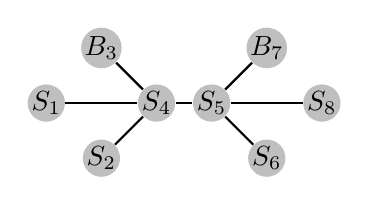
\begin{tikzpicture}[scale=0.7]
    % Draw a 7,11 network
    % First we draw the vertices
    \foreach \pos/\name in {{(1,2)/S_1}, {(2,1)/S_2}, {(2,3)/B_3}, {(5,1)/S_6}, {(5,3)/B_7}, {(6,2)/S_8}, {(3,2)/S_4}, {(4,2)/S_5}}
        \node[vertex] (\name) at \pos {$\name$};
    
%    \foreach \pos/\name in {{(3,2)/S_4}, {(4,2)/S_5}}
%    \node[selected vertex] (\name) at \pos {$\name$};
    
    % Connect vertices with edges 
    \foreach \source/ \dest in {S_1/S_4, S_2/S_4,B_3/S_4,S_4/S_5, S_5/S_6, S_5/B_7, S_5/S_8}
        \path[edge] (\source) -- (\dest) ;
        
\end{tikzpicture}
\end{center}
\end{itemize}

\begin{itemize}
\item Equilibrium path
\begin{itemize}
\item 
\alt<2>
{
At \textcolor{blue}{$t=2$}, 
\begin{table}[h]
\begin{tabular}{ll }
S-type 4 & $(\overbrace{\alert{p},n,\alert{p},\alert{p},\alert{p},n,\alert{p},\alert{p}}^{8})$\\
S-type 5 & $(\overbrace{\alert{p},n,\alert{p},\alert{p},\alert{p},n,\alert{p},\alert{p}}^{8})$\\
S-type 1,2,6,8 & $\emptyset$
\end{tabular}
\end{table}
}
{
At \textcolor{blue}{$t=1$}, 
\begin{table}[h]
\begin{tabular}{ll l}
S-type 4 & $(\overbrace{n,n,n,\alert{p},\alert{p},n,\alert{p},\alert{p}}^{8})$\\
S-type 5 & $(\overbrace{\alert{p},n,\alert{p},\alert{p},\alert{p},n,n,n}^{8})$ \\
S-type 1,2,6,8 & $\emptyset$
\end{tabular}
\end{table}
}

\pause
\item At \textcolor{blue}{$t=3$}, all S-types play \textbf{p}, then game ends.

\end{itemize}

\end{itemize}



\end{frame}


\begin{frame}
  \frametitle{$k$-Threshold game augmented by $T$-round \alt<2->{costly talk}{cheap talk}}

\onslide<2->{ If there is a fixed cost $\epsilon$ to send the letter...}

\begin{itemize}

\item Off-path strategy
\begin{itemize}
\item If S-type 4 (or 5) make detectable deviation \alt<2->{(e.g. wrong sentence, playing $\emptyset$)}{(e.g. wrong sentence)}

$\Rightarrow$ others play \alt<2->{$\emptyset$}{\textbf{n}} and then \textbf{n}.
\item If S-type 4 (or 5) make undetectable deviation $\Rightarrow$ he is facing a possibility of failure to coordinate.
\end{itemize}
\item Off-path belief
\begin{itemize}
\item Detectable deviation $\Rightarrow$ believing that all players outside neighborhood are B-types. 
\end{itemize}
\end{itemize}

\onslide<3>{
\alert{So}, when \textcolor{red}{$\epsilon$ is small enough and $T$ is large enough}, an weak equilibrium can be constructed \alert{when $\epsilon$ is independent from messages}.}


\end{frame}





\begin{frame}
   \frametitle{$k$-Threshold game augmented by $T$-round costly talk}
\framesubtitle{Free Rider Problem}

\alert{However}, if $\epsilon$ is \alert{not independent from messages}, then a \alert{Free Rider Problem} may occur.
\begin{itemize}
\item Suppose $\epsilon$ \alert{$\downarrow$} when announce \alert{more} S-types in the \alert{$1^{st}$} round.
\item $k=5$, $n=8$ and $T=2$.
\item $G$ and $\theta$=
\begin{center}
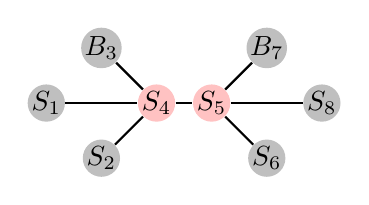
\begin{tikzpicture}[scale=0.7]
    % Draw a 7,11 network
    % First we draw the vertices
    \foreach \pos/\name in {{(1,2)/S_1}, {(2,1)/S_2}, {(2,3)/B_3}, {(5,1)/S_6}, {(5,3)/B_7}, {(6,2)/S_8}}
        \node[vertex] (\name) at \pos {$\name$};
    
    \foreach \pos/\name in {{(3,2)/S_4}, {(4,2)/S_5}}
    \node[selected vertex] (\name) at \pos {$\name$};
    
    % Connect vertices with edges 
    \foreach \source/ \dest in {S_1/S_4, S_2/S_4,B_3/S_4,S_4/S_5, S_5/S_6, S_5/B_7, S_5/S_8}
        \path[edge] (\source) -- (\dest) ;
        
\end{tikzpicture}
\end{center}



\end{itemize}

\begin{enumerate}
\item S-type \alert{4} and S-type \alert{5} will deviate from truthfully announcement.
\item Why? They will report more S-types to save costs in the 1st round and ``wait for'' each others' truthfully announcement (Free Rider Problem).
\end{enumerate}


\end{frame}




\begin{frame}
\frametitle{Result 2: APEX for $k<n$}
\begin{theorem}[\alert{$k< n$}]
If $k<n$, then if network is a \alert{tree}, if prior $\pi$ has \alert{full support on strong connectedness}, then an APEX WPBE {exists} whenever discount factor is sufficiently high.
\end{theorem}

Sketch of proof:
\begin{enumerate}
\item \underline{The Free Rider Problem may exist in tree networks, but it can be solved}.
\item Detectable deviation $\Rightarrow$ playing \textbf{n} forever (by off-path belief).
\item Undetectable deviation $\Rightarrow$ facing a possibility of coordination failure.
\item Any deviation will let APEX fail with positive probability.
\item APEX outcome gives maximum ex-post continuation pay-off after $T$.
\item Sufficiently high discount factor will impede deviation.
\end{enumerate}



\end{frame}


\section{Discussion}
\subsection{Discussion}





%\begin{frame}
%\frametitle{Extension}
%\framesubtitle{Pay-off as a signal}
%\begin{enumerate}
%
%\item payoff is perfectly observed
%\begin{itemize}
%\item Play \textbf{p} in the first period, then the relevant information revealed.
%
%\end{itemize}
%\item payoff is noisy
%\begin{itemize}
%\item With full support assumption, the existing equilibrium is APEX.
%\item Ex: 
%\begin{itemize}
%\item $u_{s_i}(a, \alert{y})$ is dependent on a random variable $\alert{y}\in \{y_1,y_2\}$
%\item full support:
%\begin{eqnarray*}
%p_{1,\geq k} &=& \mathrm {Pr}(y=y_1|\#\textbf{p}\geq k)>0 \\
%p_{1,<k} &=& \mathrm {Pr}(y=y_1|\#\textbf{p}< k)>0 \\
%p_{2,\geq k} &=& \mathrm {Pr}(y=y_2|\#\textbf{p}\geq k)>0 \\
%p_{2,<k} &=& \mathrm {Pr}(y=y_2|\#\textbf{p}< k)>0 
%\end{eqnarray*}
%\item S-type: \underline{the expected payoff on $\#\textbf{p}\geq k$} strictly larger than \underline{the expected payoff on $\#\textbf{p}< k$}
%\end{itemize}
%
%
%
%
%\end{itemize}
%
%
%\end{enumerate}
%
%
%\end{frame}


\section{Future Works}
\subsection{Future Works}


\begin{frame}

\frametitle{Further works}


\begin{enumerate}
\item Tackle cyclic networks.
\item Look for a general model such that a finite-time communication protocol exists and this protocol can be extended to an equilibrium.

\end{enumerate}
\end{frame}





\end{document}
